\documentclass[tikz, border=2mm]{standalone}
\usepackage{amsmath}
\usepackage{amssymb}
\usepackage{mathptmx} % Times font
\usetikzlibrary{shapes.geometric, arrows.meta, positioning, fit, backgrounds, calc}

\begin{document}
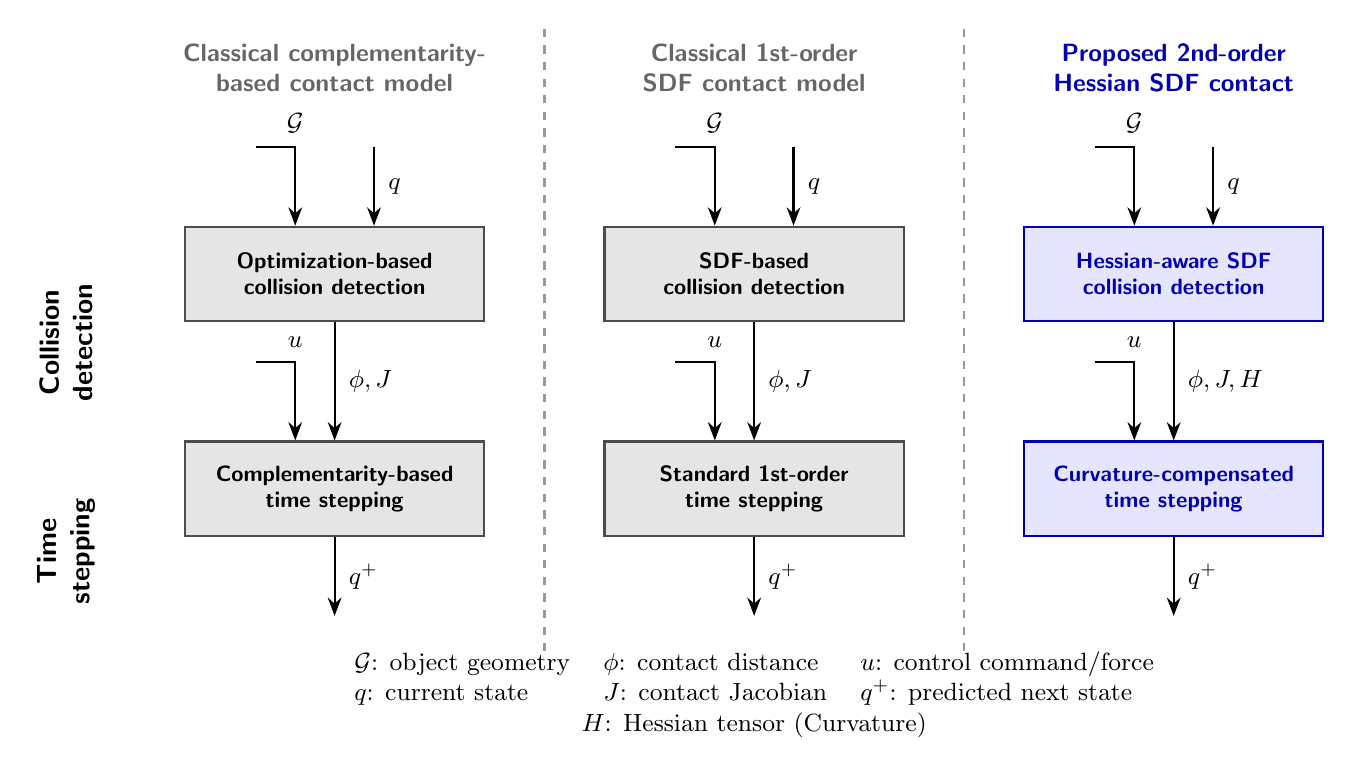
\begin{tikzpicture}[
    >=Stealth,
    node distance=1.5cm and 2.5cm,
    box/.style={rectangle, draw=black!70, thick, minimum width=3.8cm, minimum height=1.2cm, align=center, fill=black!10, font=\footnotesize\sffamily\bfseries},
    box_prop/.style={box, draw=blue!70!black, fill=blue!10, text=blue!70!black},
    title/.style={font=\small\bfseries\sffamily, align=center, text=black!60, minimum height=1cm},
    title_prop/.style={title, text=blue!70!black},
    arrow/.style={->, thick, >=Stealth},
    label_node/.style={font=\small\itshape}
]

% --- Column 1 (Mesh) ---
\node[box] (cd_mesh) {Optimization-based\\collision detection};
\node[title, above=1.5cm of cd_mesh] (title_mesh) {Classical complementarity-\\based contact model};
\node[box, below=1.5cm of cd_mesh] (ts_mesh) {Complementarity-based\\time stepping};

% --- Column 2 (Classical SDF) ---
\node[box, right=1.5cm of cd_mesh] (cd_sdf) {SDF-based\\collision detection};
\node[title, above=1.5cm of cd_sdf] (title_sdf) {Classical 1st-order\\SDF contact model};
\node[box, below=1.5cm of cd_sdf] (ts_sdf) {Standard 1st-order\\time stepping};

% --- Column 3 (Proposed SDF) ---
\node[box_prop, right=1.5cm of cd_sdf] (cd_prop) {Hessian-aware SDF\\collision detection};
\node[title_prop, above=1.5cm of cd_prop] (title_prop) {Proposed 2nd-order\\Hessian SDF contact};
\node[box_prop, below=1.5cm of cd_prop] (ts_prop) {Curvature-compensated\\time stepping};

% --- Side Labels ---
\node[left=1.5cm of cd_mesh, rotate=90, font=\normalsize\bfseries\sffamily, align=center] (label_cd) {Collision\\detection};
\node[left=1.5cm of ts_mesh, rotate=90, font=\normalsize\bfseries\sffamily, align=center] (label_ts) {Time\\stepping};

% --- Arrows for Mesh ---
% Inputs to CD
\coordinate (g_mesh_in) at ([xshift=-1.0cm, yshift=1.0cm]cd_mesh.north);
\draw[arrow] (g_mesh_in) -| node[above=0.05cm, font=\small] {$\mathcal{G}$} ([xshift=-0.5cm]cd_mesh.north);
\coordinate (q_mesh_in) at ([xshift=0.5cm, yshift=1.0cm]cd_mesh.north);
\draw[arrow] (q_mesh_in) -- node[right=0.05cm, font=\small] {$q$} ([xshift=0.5cm]cd_mesh.north);

% CD to TS
\draw[arrow] (cd_mesh) -- node[right=0.05cm, font=\small] {$\phi, J$} (ts_mesh);

% Inputs to TS
\coordinate (u_mesh_in) at ([xshift=-1.0cm, yshift=1.0cm]ts_mesh.north);
\draw[arrow] (u_mesh_in) -| node[above=0.05cm, font=\small] {$u$} ([xshift=-0.5cm]ts_mesh.north);

% Output of TS
\coordinate (q_mesh_out) at ([yshift=-1.0cm]ts_mesh.south);
\draw[arrow] (ts_mesh) -- node[right=0.05cm, font=\small] {$q^+$} (q_mesh_out);

% --- Arrows for SDF ---
% Inputs to CD
\coordinate (g_sdf_in) at ([xshift=-1.0cm, yshift=1.0cm]cd_sdf.north);
\draw[arrow] (g_sdf_in) -| node[above=0.05cm, font=\small] {$\mathcal{G}$} ([xshift=-0.5cm]cd_sdf.north);
\coordinate (q_sdf_in) at ([xshift=0.5cm, yshift=1.0cm]cd_sdf.north);
\draw[arrow] (q_sdf_in) -- node[right=0.05cm, font=\small] {$q$} ([xshift=0.5cm]cd_sdf.north);

% CD to TS
\draw[arrow] (cd_sdf) -- node[right=0.05cm, font=\small] {$\phi, J$} (ts_sdf);

% Inputs to TS
\coordinate (u_sdf_in) at ([xshift=-1.0cm, yshift=1.0cm]ts_sdf.north);
\draw[arrow] (u_sdf_in) -| node[above=0.05cm, font=\small] {$u$} ([xshift=-0.5cm]ts_sdf.north);

% Output of TS
\coordinate (q_sdf_out) at ([yshift=-1.0cm]ts_sdf.south);
\draw[arrow] (ts_sdf) -- node[right=0.05cm, font=\small] {$q^+$} (q_sdf_out);

% --- Arrows for Proposed ---
% Inputs to CD
\coordinate (g_prop_in) at ([xshift=-1.0cm, yshift=1.0cm]cd_prop.north);
\draw[arrow] (g_prop_in) -| node[above=0.05cm, font=\small] {$\mathcal{G}$} ([xshift=-0.5cm]cd_prop.north);
\coordinate (q_prop_in) at ([xshift=0.5cm, yshift=1.0cm]cd_prop.north);
\draw[arrow] (q_prop_in) -- node[right=0.05cm, font=\small] {$q$} ([xshift=0.5cm]cd_prop.north);

% CD to TS
\draw[arrow] (cd_prop) -- node[right=0.05cm, font=\small] {$\phi, J, H$} (ts_prop);

% Inputs to TS
\coordinate (u_prop_in) at ([xshift=-1.0cm, yshift=1.0cm]ts_prop.north);
\draw[arrow] (u_prop_in) -| node[above=0.05cm, font=\small] {$u$} ([xshift=-0.5cm]ts_prop.north);

% Output of TS
\coordinate (q_prop_out) at ([yshift=-1.0cm]ts_prop.south);
\draw[arrow] (ts_prop) -- node[right=0.05cm, font=\small] {$q^+$} (q_prop_out);

% --- Separators ---
\draw[dashed, thick, black!40] ($(cd_mesh.north east)!0.5!(cd_sdf.north west) + (0, 2.5cm)$) -- ++(0, -8.0cm);
\draw[dashed, thick, black!40] ($(cd_sdf.north east)!0.5!(cd_prop.north west) + (0, 2.5cm)$) -- ++(0, -8.0cm);

% --- Legend ---
\node[below=2.0cm of ts_sdf, anchor=center, font=\small] (legend) {
    \begin{tabular}{lll}
    $\mathcal{G}$: object geometry & $\phi$: contact distance & $u$: control command/force \\
    $q$: current state & $J$: contact Jacobian & $q^+$: predicted next state \\
    \multicolumn{3}{c}{$H$: Hessian tensor (Curvature)}
    \end{tabular}
};

\end{tikzpicture}
\end{document}